\documentclass{article}

\usepackage{graphicx} % Required for inserting images
\usepackage{parskip}                              % no indent
\usepackage{setspace}                             % line spacing, we'll use \setstretch{1.2}
\usepackage[a4paper, bottom=3cm]{geometry}

% TEXT

\usepackage[T1]{fontenc}                        % letters such as ç, ò, etc

\usepackage[backend=biber, style=authoryear]{biblatex}
\addbibresource{refs.bib}

\usepackage{mathtools,amsmath,amssymb,amsthm}   % math symbols, and theorems
\usepackage{dsfont}                             % indicator function
\usepackage{siunitx}                            % writing units (15 h, 10 kg, etc)
\usepackage{xltabular}                          % for xltabular environment
\usepackage{hyperref}
    \hypersetup{
        colorlinks=true,
        linkcolor=blue,
        citecolor=blue,
    }


% TEXT FORMATTING
\usepackage[dvipsnames]{xcolor}                   % colors for the hyperlinks
% \definecolor{purplecite}{RGB}{202, 97, 228}         % define new color
\usepackage{enumitem}   

\newcommand {\Z}{\mathbb{Z}}                    % shortcuts for symbols
\newcommand {\R}{\mathbb{R}}
\newcommand {\diff}{\mathrm{d}}

\newtheorem{theorem}{Theorem}                   % theorem environments
\newtheorem{definition}{Definition}
\newtheorem{proposition}{Proposition}
\newtheorem*{proposition*}{Proposition}
\newtheorem{lemma}{Lemma}
\newtheorem{remark}{Remark}
\newtheorem{corollary}{Corollary}
\newtheorem{example}{Example}
\newtheorem{codedef}{Code}
\newtheorem{program}{Program}
\newtheorem{notation}{Notation}





\begin{document}


{\huge\centering 3D modelling of confined gastruloid aggregates\par}

\tableofcontents

\vspace{1em}

\section{The gastruloid physical model}

\begin{definition}
    The \textbf{equations of motion} are given by
    \begin{equation*}
        {\mathbf{v}}_i = \frac{1}{{\lambda} n_i} \sum_j {\mathbf{F}}_{ij} + \frac{\alpha}{n_i} \sum_j {\mathbf{v}}_j \,.
    \end{equation*}
    \textbf{Cellular forces} are given by
    \begin{equation*}
        \mathbf{F}_{ij}(s_i, s_j, d_{ij}) = f(d_{ij})\, \hat{\mathbf{r}}_{ij} \cdot
        \begin{cases}
            F_\text{rep}^{(s_i, s_j)}, & \text{if } d_{ij} \leq 2r \\
            F_\text{att}^{(s_i, s_j)}, & \text{if } 2r < d_{ij} < 2\mu r \\
            0, & \text{otherwise} \,,
        \end{cases}
    \end{equation*}
    where $s_i,s_j \in\{A,B,C\}$, 
    ${d}_{ij} = {|\mathbf{x}_i - \mathbf{x}_j|}$,
    $\hat{\mathbf{r}}_{ij} = \frac{\mathbf{x}_i - \mathbf{x}_j}{|\mathbf{x}_i - \mathbf{x}_j|}$, 
    and 
    $$f(d_{ij}) = \left(\frac{2r}{d_{ij}} - 1\right)\left(\frac{2\mu r}{d_{ij}} - 1\right) \,.$$
\end{definition}

\begin{remark}
    In the code we set $\hat\alpha=\lambda\alpha$ and so
    \begin{equation*}
        {\mathbf{v}}_i = \frac{1}{{\lambda} n_i}\left( \sum_j {\mathbf{F}}_{ij} + \alpha \sum_j {\mathbf{v}}_j \right) \,.
    \end{equation*}
\end{remark}

\begin{definition}
    The \textbf{division time} is chosen uniformly at random from
    \begin{equation*}
        \text{U}\left(\tau_{div}(1-\sigma_{div}),\tau_{div}(1+\sigma_{div})\right) \,.
    \end{equation*}
\end{definition}

\begin{definition}
    The \textbf{transition rates} depend on the proportion of cells in state $A$, namely
    \begin{align}
        \begin{aligned}
            r_{A\rightarrow B}^{(i)}&=\frac{p}{1+\phi_A/K}\\
            r_{B\rightarrow C}^{(i)}&=\frac{q}{1+\phi_A/K} \,.
        \end{aligned}
    \end{align}
\end{definition}


\section{Description of the experiment}

In the original experiment as follows.

First, we grow and differentiate a gastruloid aggregate before polarisation begins. If we use the three-state cell description used in \cite{oriola} ($A\to B\to C$), the resulting aggregate at this step is a spheroid with an outer layer of $C$ cells and a central cluster of $A,B$ cells. If we were to let this further evolve, this centroid would move away from the center to the outer layer (polsarisation).

Before this polarisation occurs, we confine this spherical aggregate inside two plates and observe different phenomena. On confinement, the result is a pancake-shaped aggregate inheriting the previous structue (an outer layer of $C$ cells and a central cluster of $A,B$ cells) but, after some time, this structure can evolve into two different phenomena. If the radius of the \textit{pancake} is not wide enough, this cluster remains in the center and all its cells eventually differentiate to $C$. However, if the radius is large enough, then we observe some pattern-like structures formed by several $AB$-clusters that spread across the whole aggregate.

We note that the same number of cells that yields patterns for a given confinement thickness may not give rise to patterns for thicker \textit{pancakes}, since their radius will be smaller.


\section{Simulations}

The main challenge of the simulations is to show the observed patterns for several confinement thicknesses and, using the same parameters, to replicate the following phenomena observed in the nonconfined gastruloid aggregates:
\begin{enumerate}
    \item Polarisation of the central cluster.
    \item Different behaviours for fusion of certain types of cells.
\end{enumerate}

In order to fit our original parameters to the experiment, we start off using the parameters exposed in Table \ref{parameters}, which have been checked by Sotiris Samatas to yield the appropiate fusion results (see Figure \ref{fusion}).

Next, we tweak this parameter set slightly in order to attain both unconfined polarisation (see Figure \ref{polarisation}) and confined patterns f(see Figure \ref{example-patterns}).

\begin{figure}
    \centering
    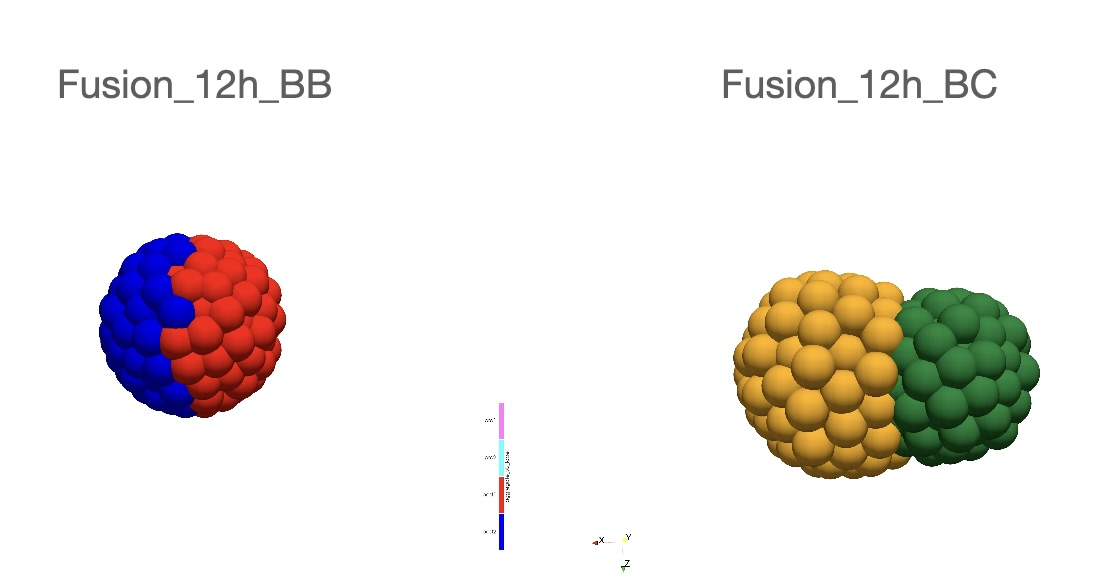
\includegraphics[width=0.5\linewidth]{figures/sotiris_fusion-edit.jpeg}
    \caption{Fusion simulations carried out by Sotiris which replicate the experimental $BB$ and $BC$ fusions.}
    \label{fusion}
\end{figure}

\begin{figure}
    \centering
    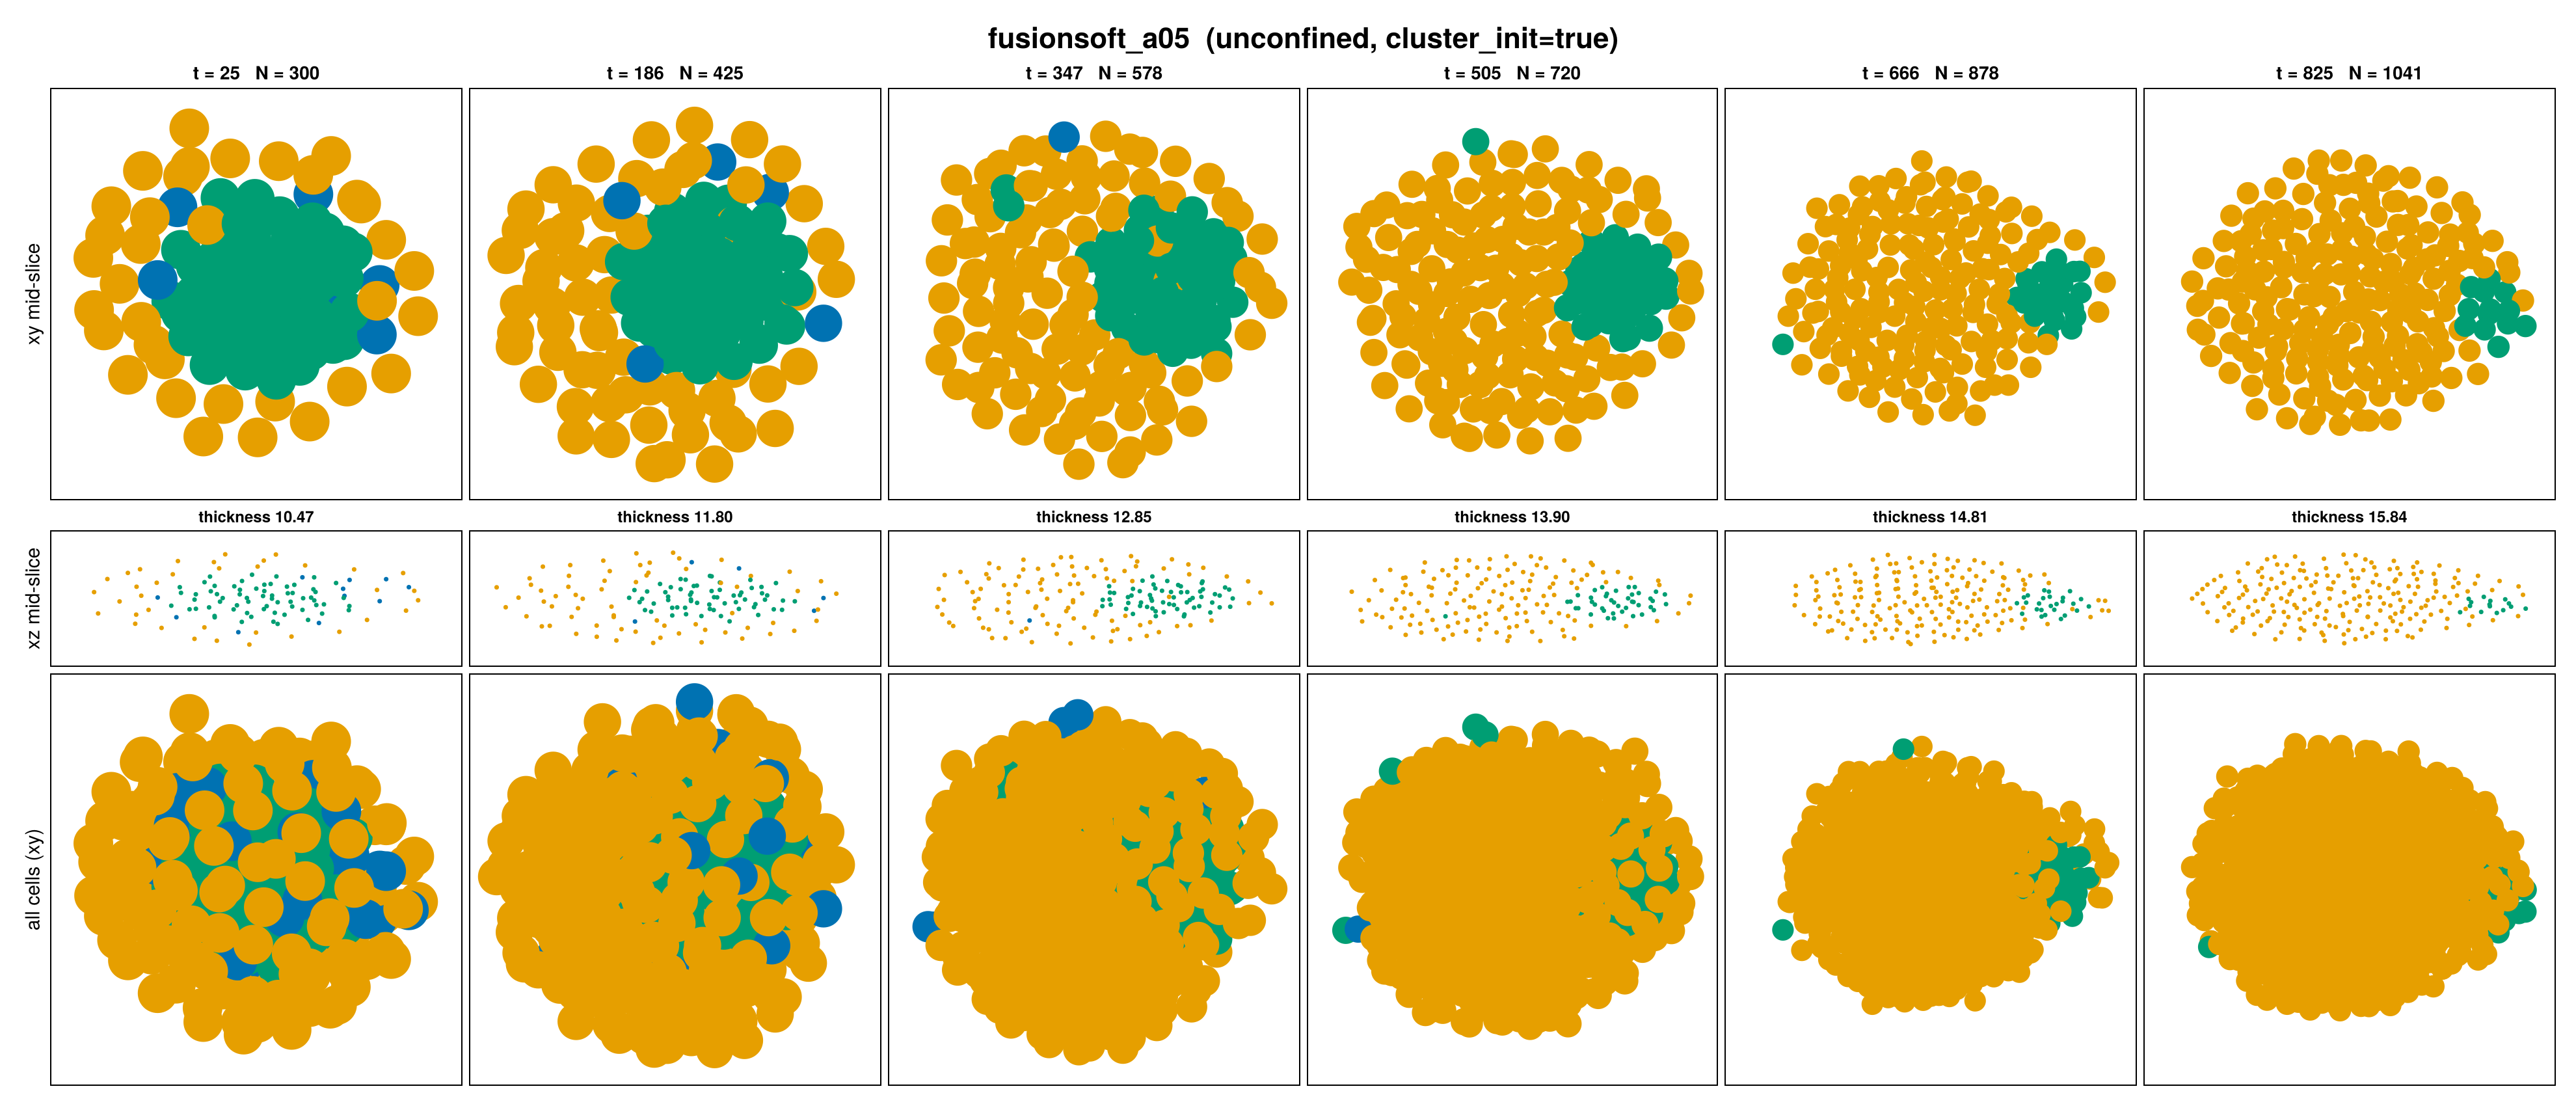
\includegraphics[width=0.8\linewidth]{figures/polsarisation.png}
    \caption{Unconfined polarisation of a 3D spherical aggregate using a 2D view. This could be plotted in 3D with no difficulty.}
    \label{polarisation}
\end{figure}

\begin{figure}
    \centering
    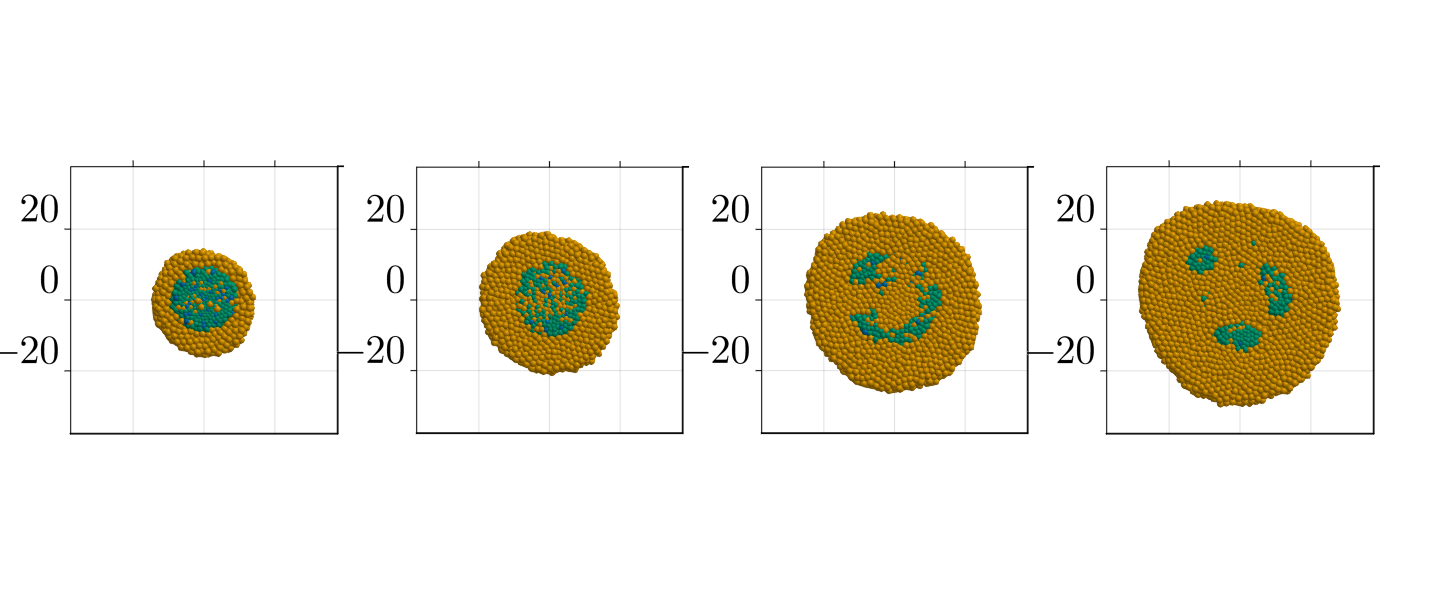
\includegraphics[width=0.8\linewidth]{figures/pancake_3layers_n2000_bottom.png}
    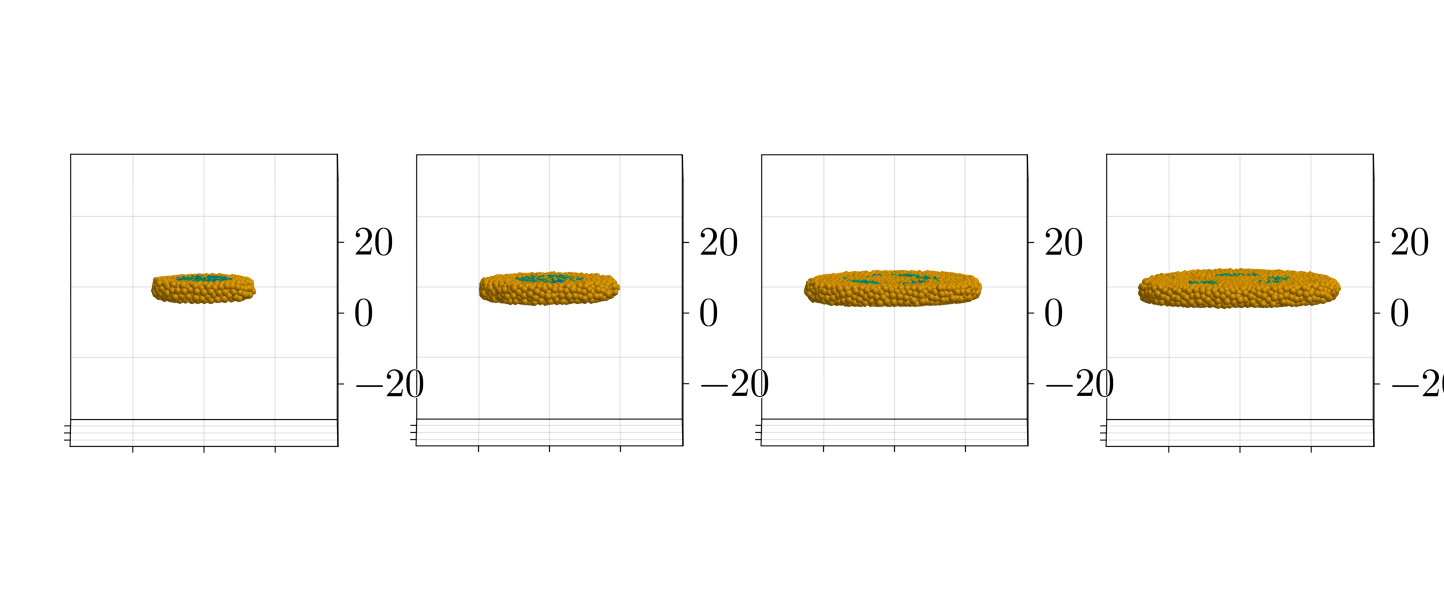
\includegraphics[width=0.8\linewidth]{figures/pancake_3layers_n2000_side.png}
    \caption{Example of patterns in a three-layer confined aggregate (that is, thickness$=3*(2r)$).}
    \label{example-patterns}
\end{figure}

We also make sure that it works for any thickness and that we get both behaviours: a stable cluster that differentiates away to $C$ if the number of cells $N$ is not large enough at the moment of the confinement, and $BC$ patterns otherwise. We define $N_0,L$ the threshold $N$ such that, for any $N>N_0,L$, a confined aggregate of thickness $L$ will yield patterns. See both behaviours for two layers and three layers in Figures \ref{2layers} and \ref{3layers}, respectively.

\begin{figure}
    \centering
    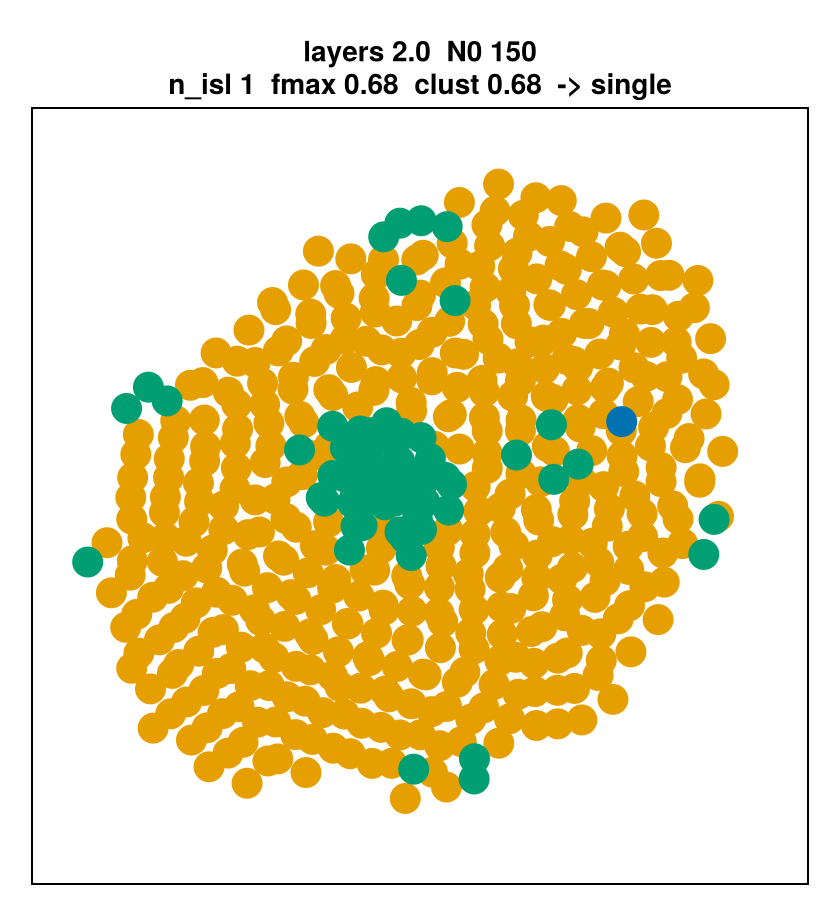
\includegraphics[width=0.23\linewidth]{figures/2layers-cluster.png}
    \hspace{3em}
    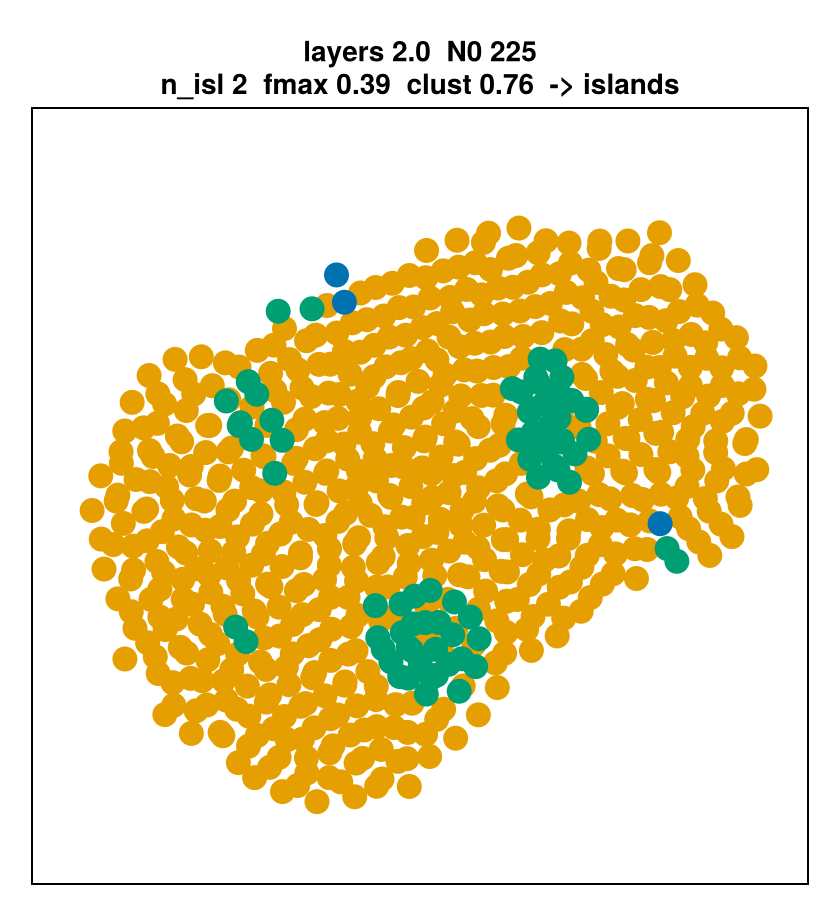
\includegraphics[width=0.23\linewidth]{figures/2layers-islands.png}
    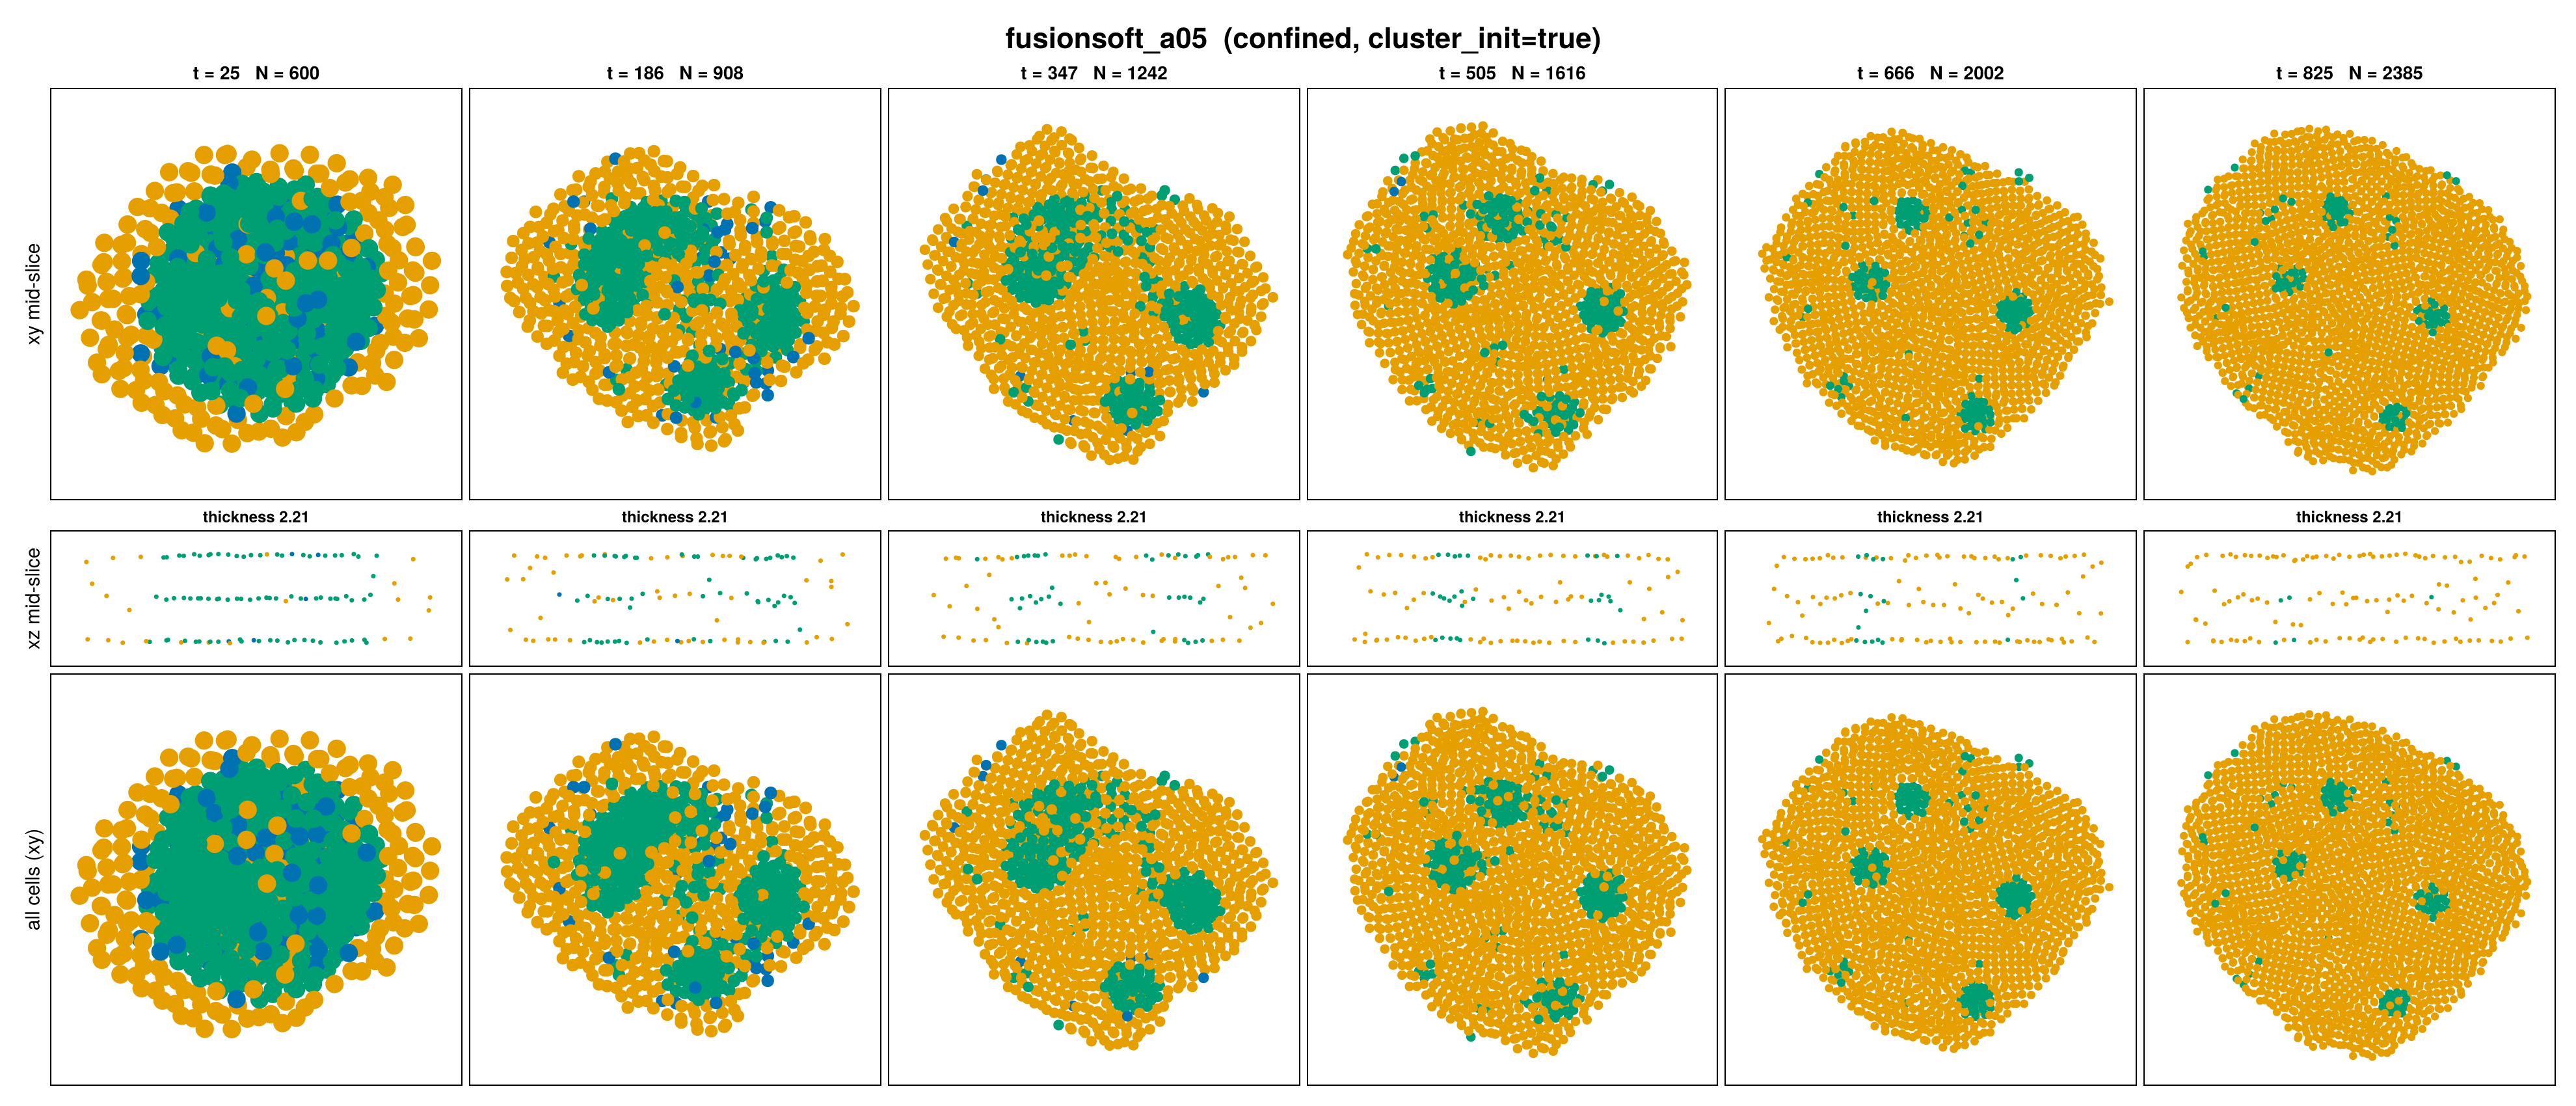
\includegraphics[width=0.8\linewidth]{figures/2layers-overtime.png}
    \caption{Two-layered aggregate with no patterns due to low $N$ and with patterns with a larger $N$.}
    \label{2layers}
\end{figure}

\begin{figure}
    \centering
    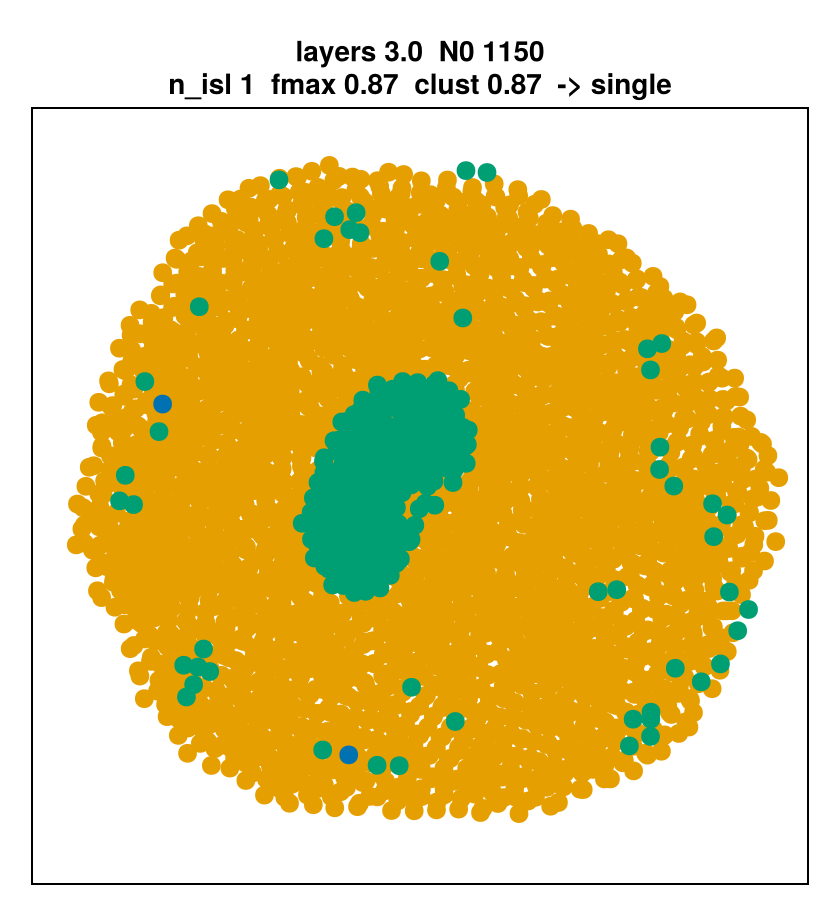
\includegraphics[width=0.23\linewidth]{figures/3layers-cluster.png}
    \hspace{3em}
    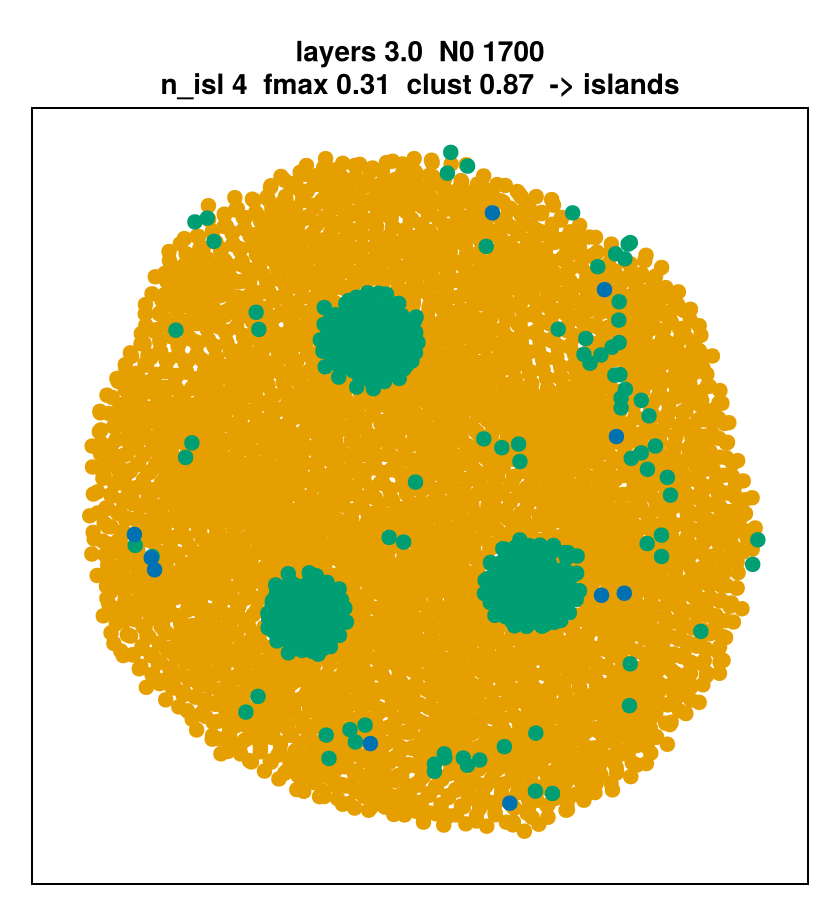
\includegraphics[width=0.23\linewidth]{figures/3layers-islands.png}
    \caption{Two-layered aggregate with no patterns due to low $N$ and with patterns with a larger $N$.}
    \label{3layers}
\end{figure}

Finally, we sketch a phase space relating the appearance of patterns, the number of layers, and the initial $N=N_0$ at the moment of squeezing, shown in Figure \ref{phase-space}

\begin{figure}
    \centering
    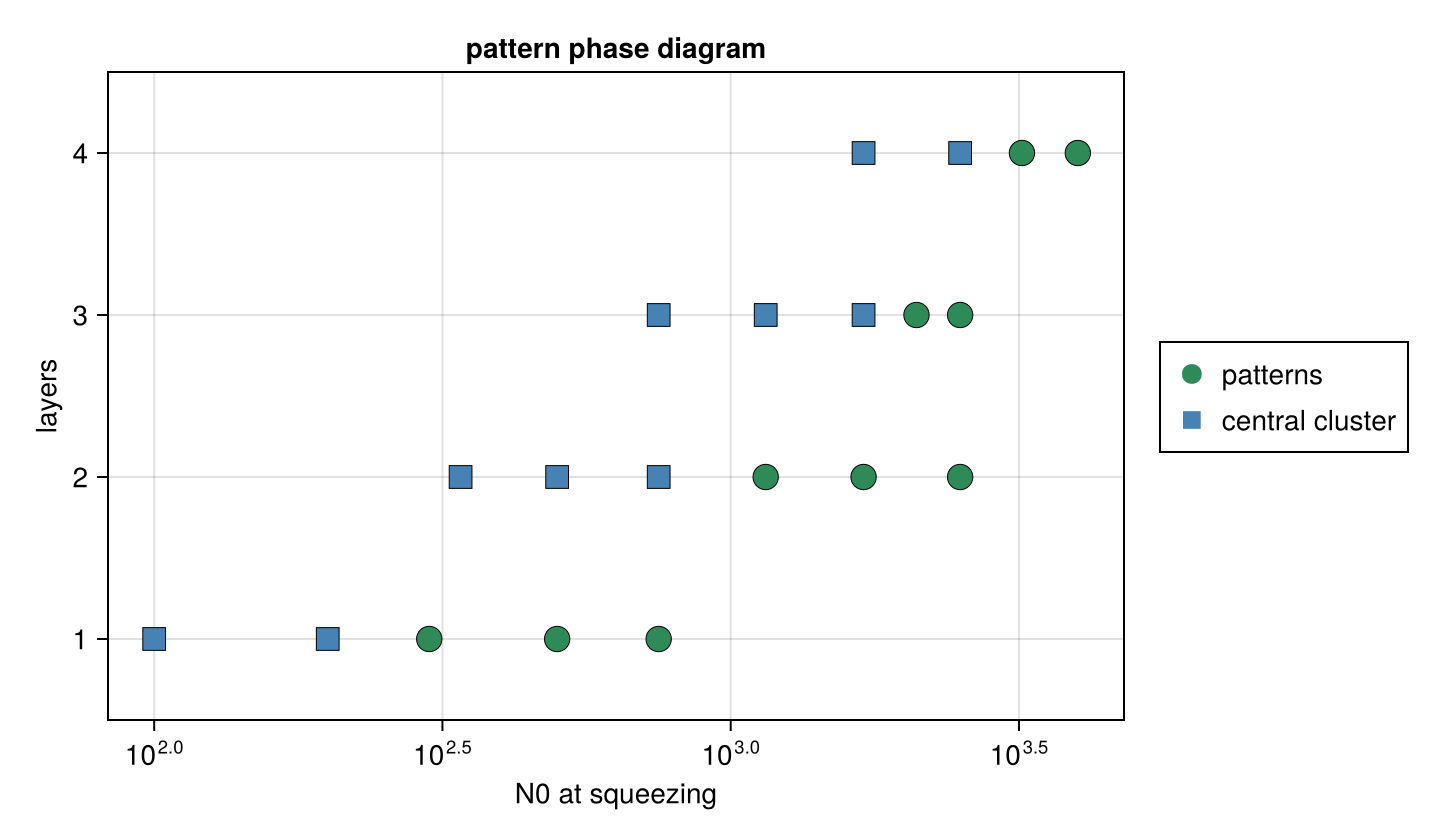
\includegraphics[width=\linewidth]{figures/Island phase space.png}
    \caption{Two-layered aggregate with no patterns due to low $N$ and with patterns with a larger $N$.}
    \label{phase-space}
\end{figure}

While tweaking the parameters, I have also observed stable behaviour that yield more concentrated patterns (much more pattern-like to the bare eye I think, but maybe not so true to the experiments). These are attached in Figure \ref{final-patterns}.

\begin{figure}
    \centering
    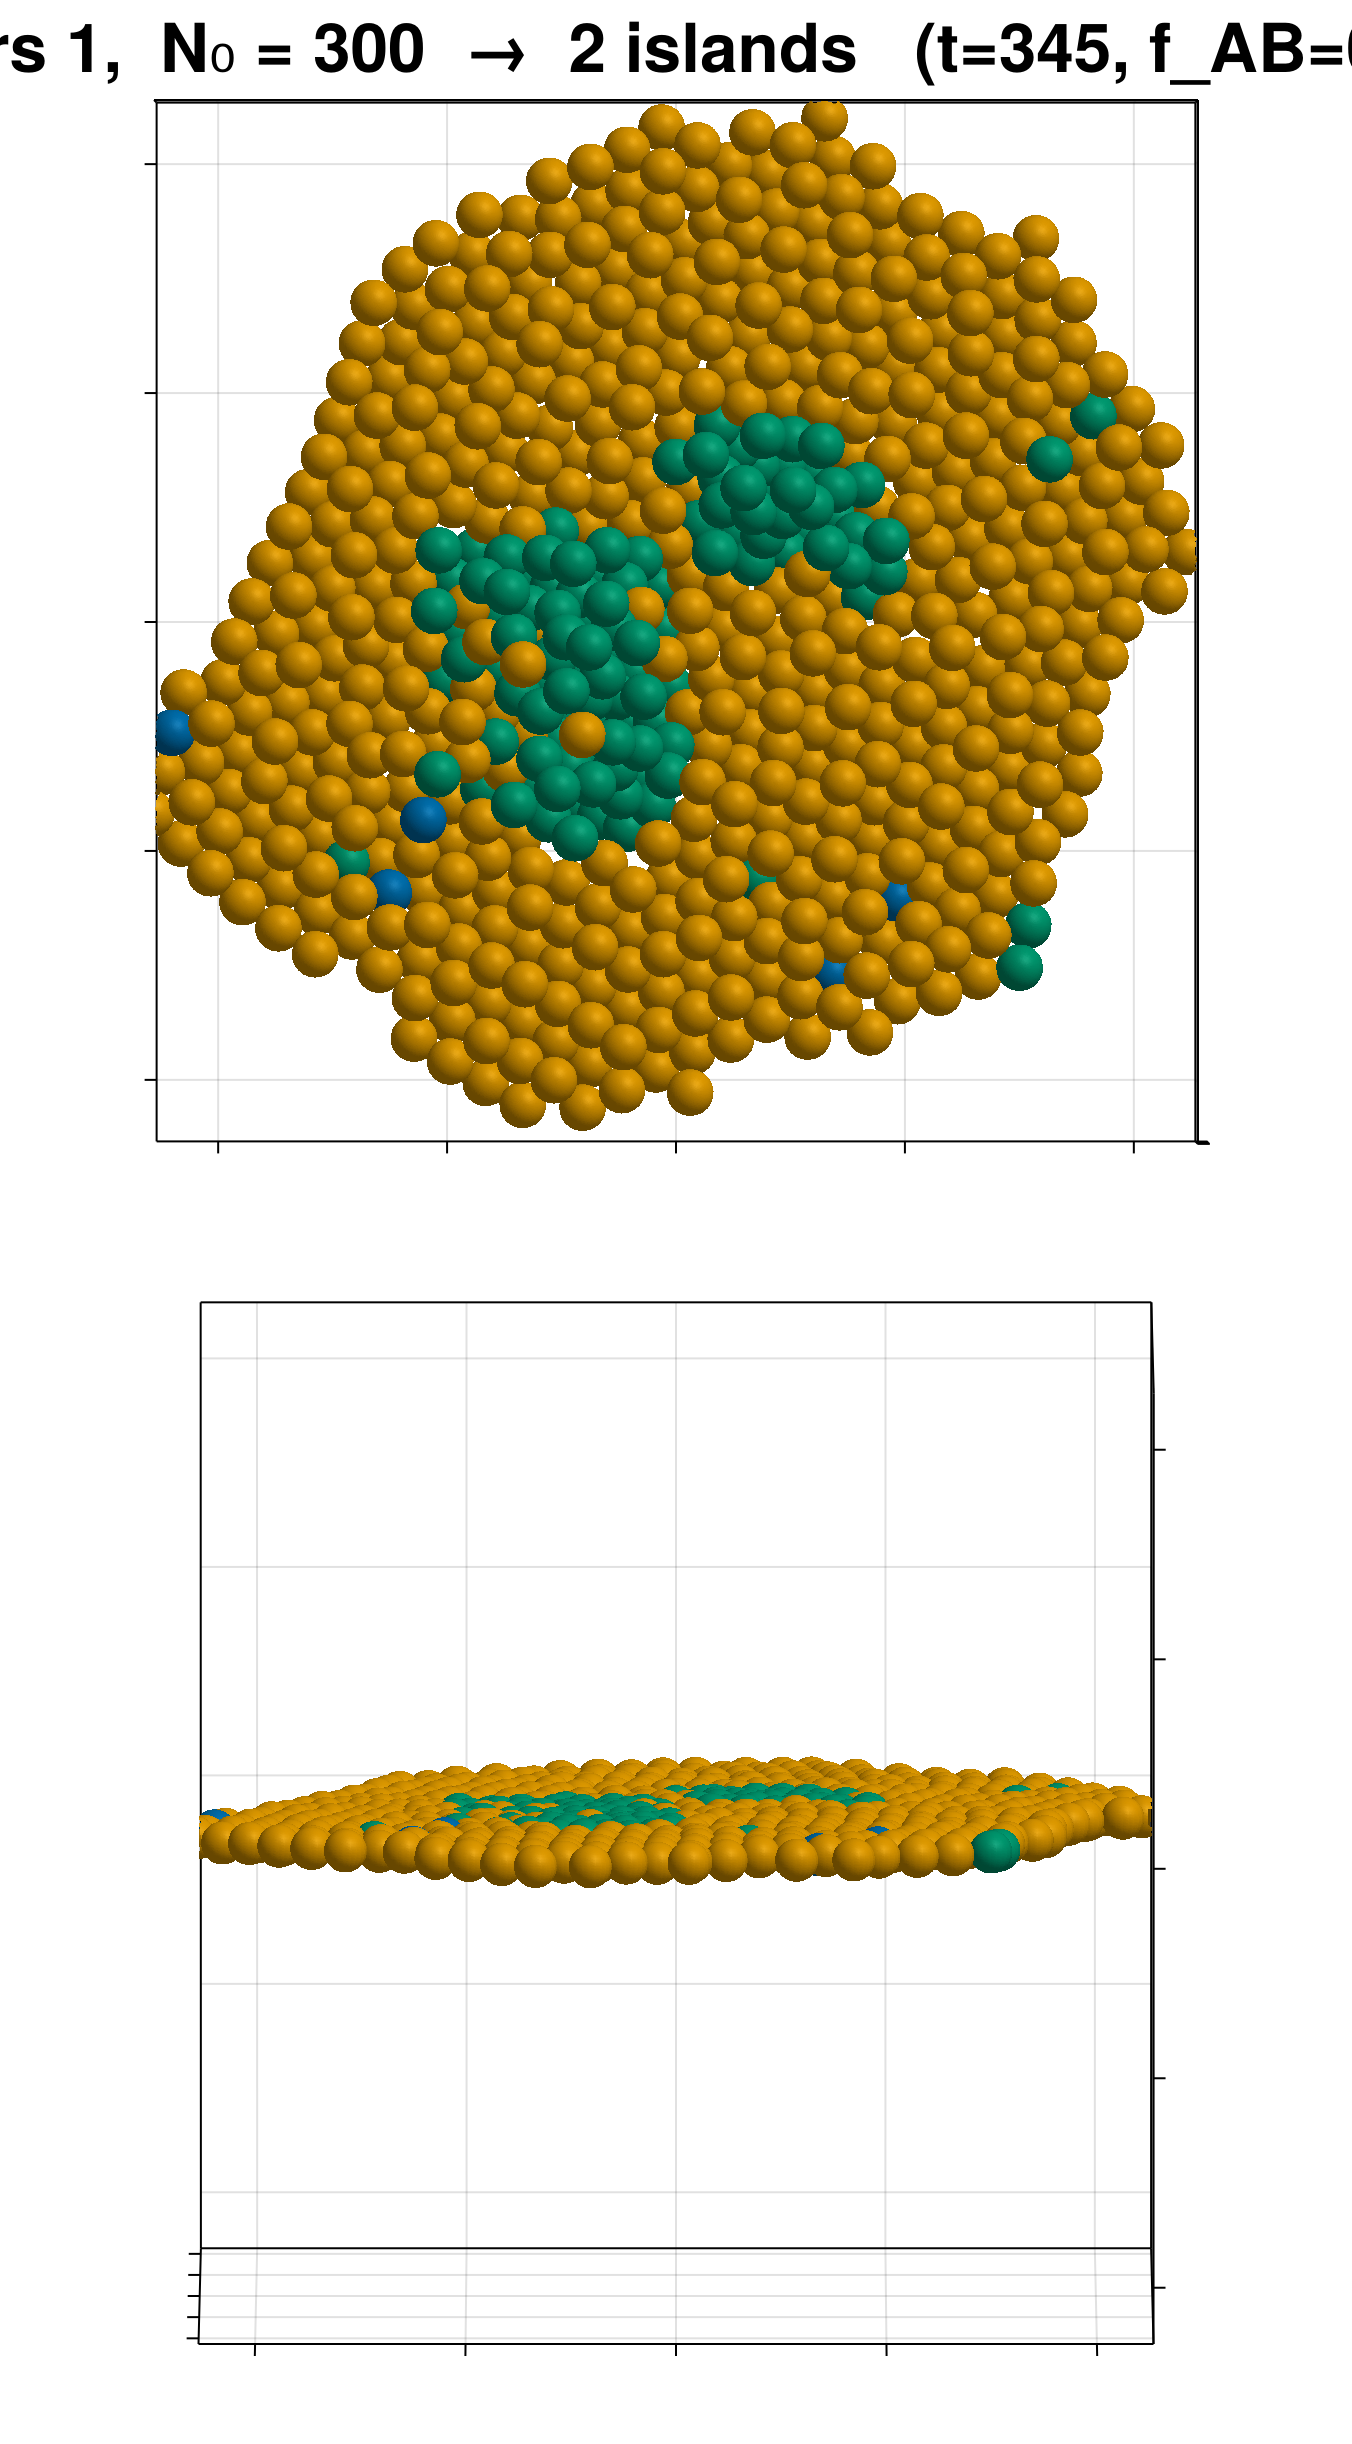
\includegraphics[width=0.2\linewidth]{figures/pattern_L1_islands_N300.png}
    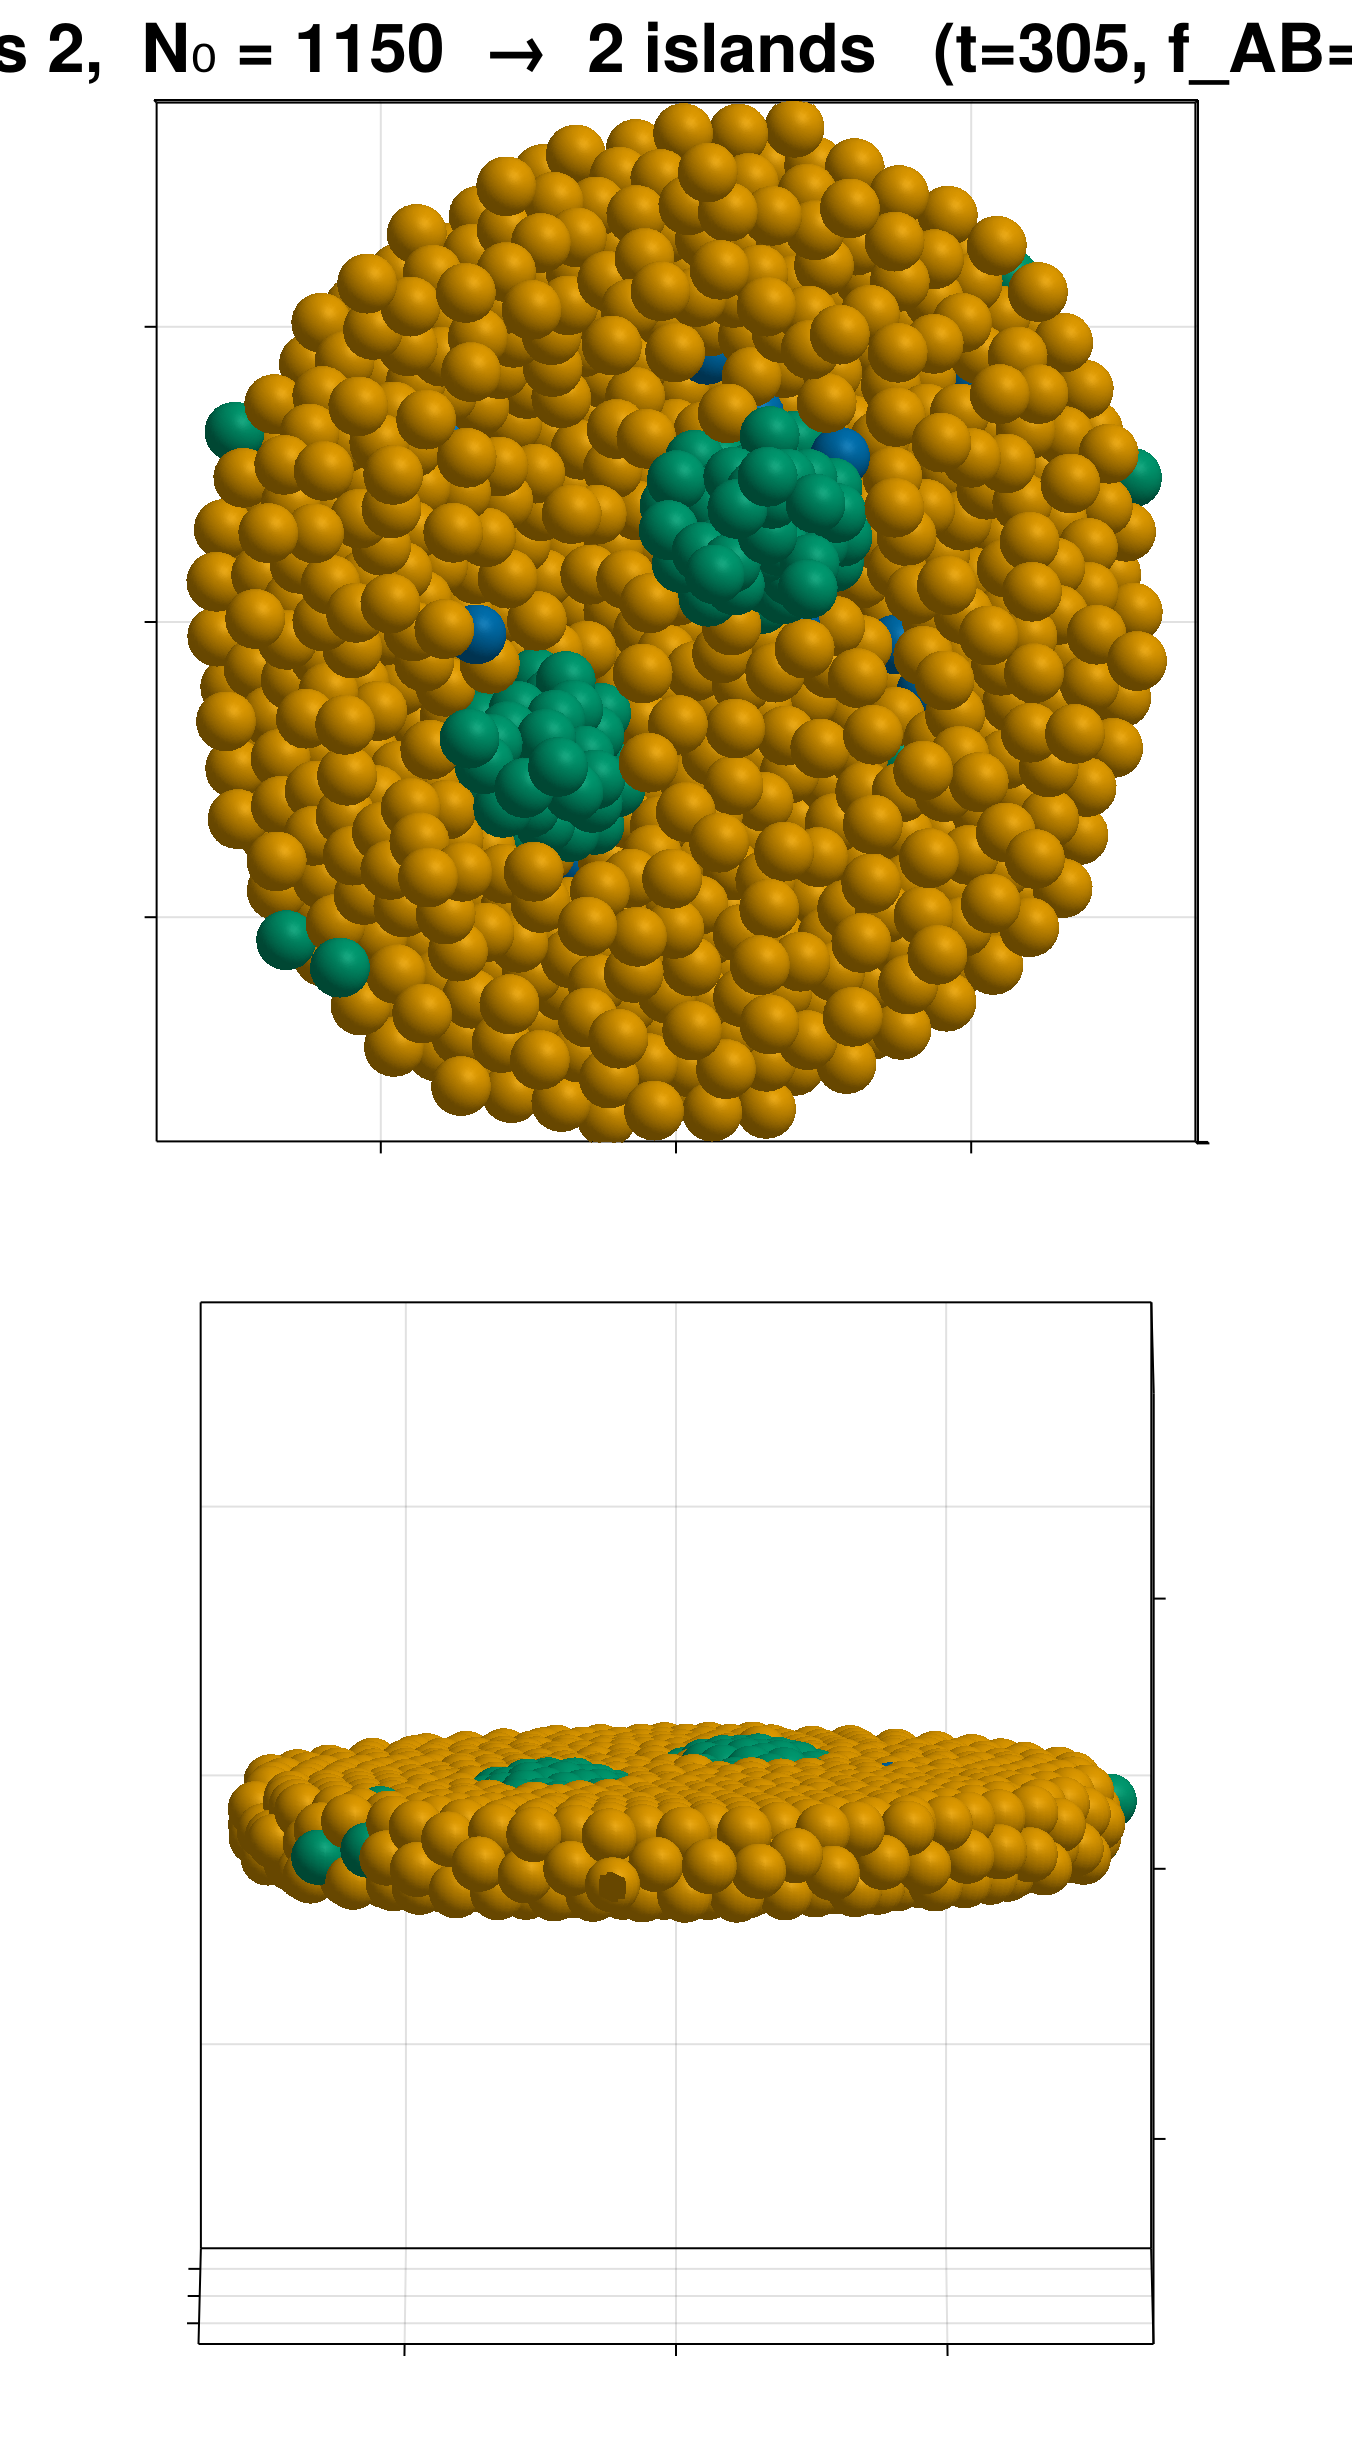
\includegraphics[width=0.2\linewidth]{figures/pattern_L2_islands_N1150.png}
    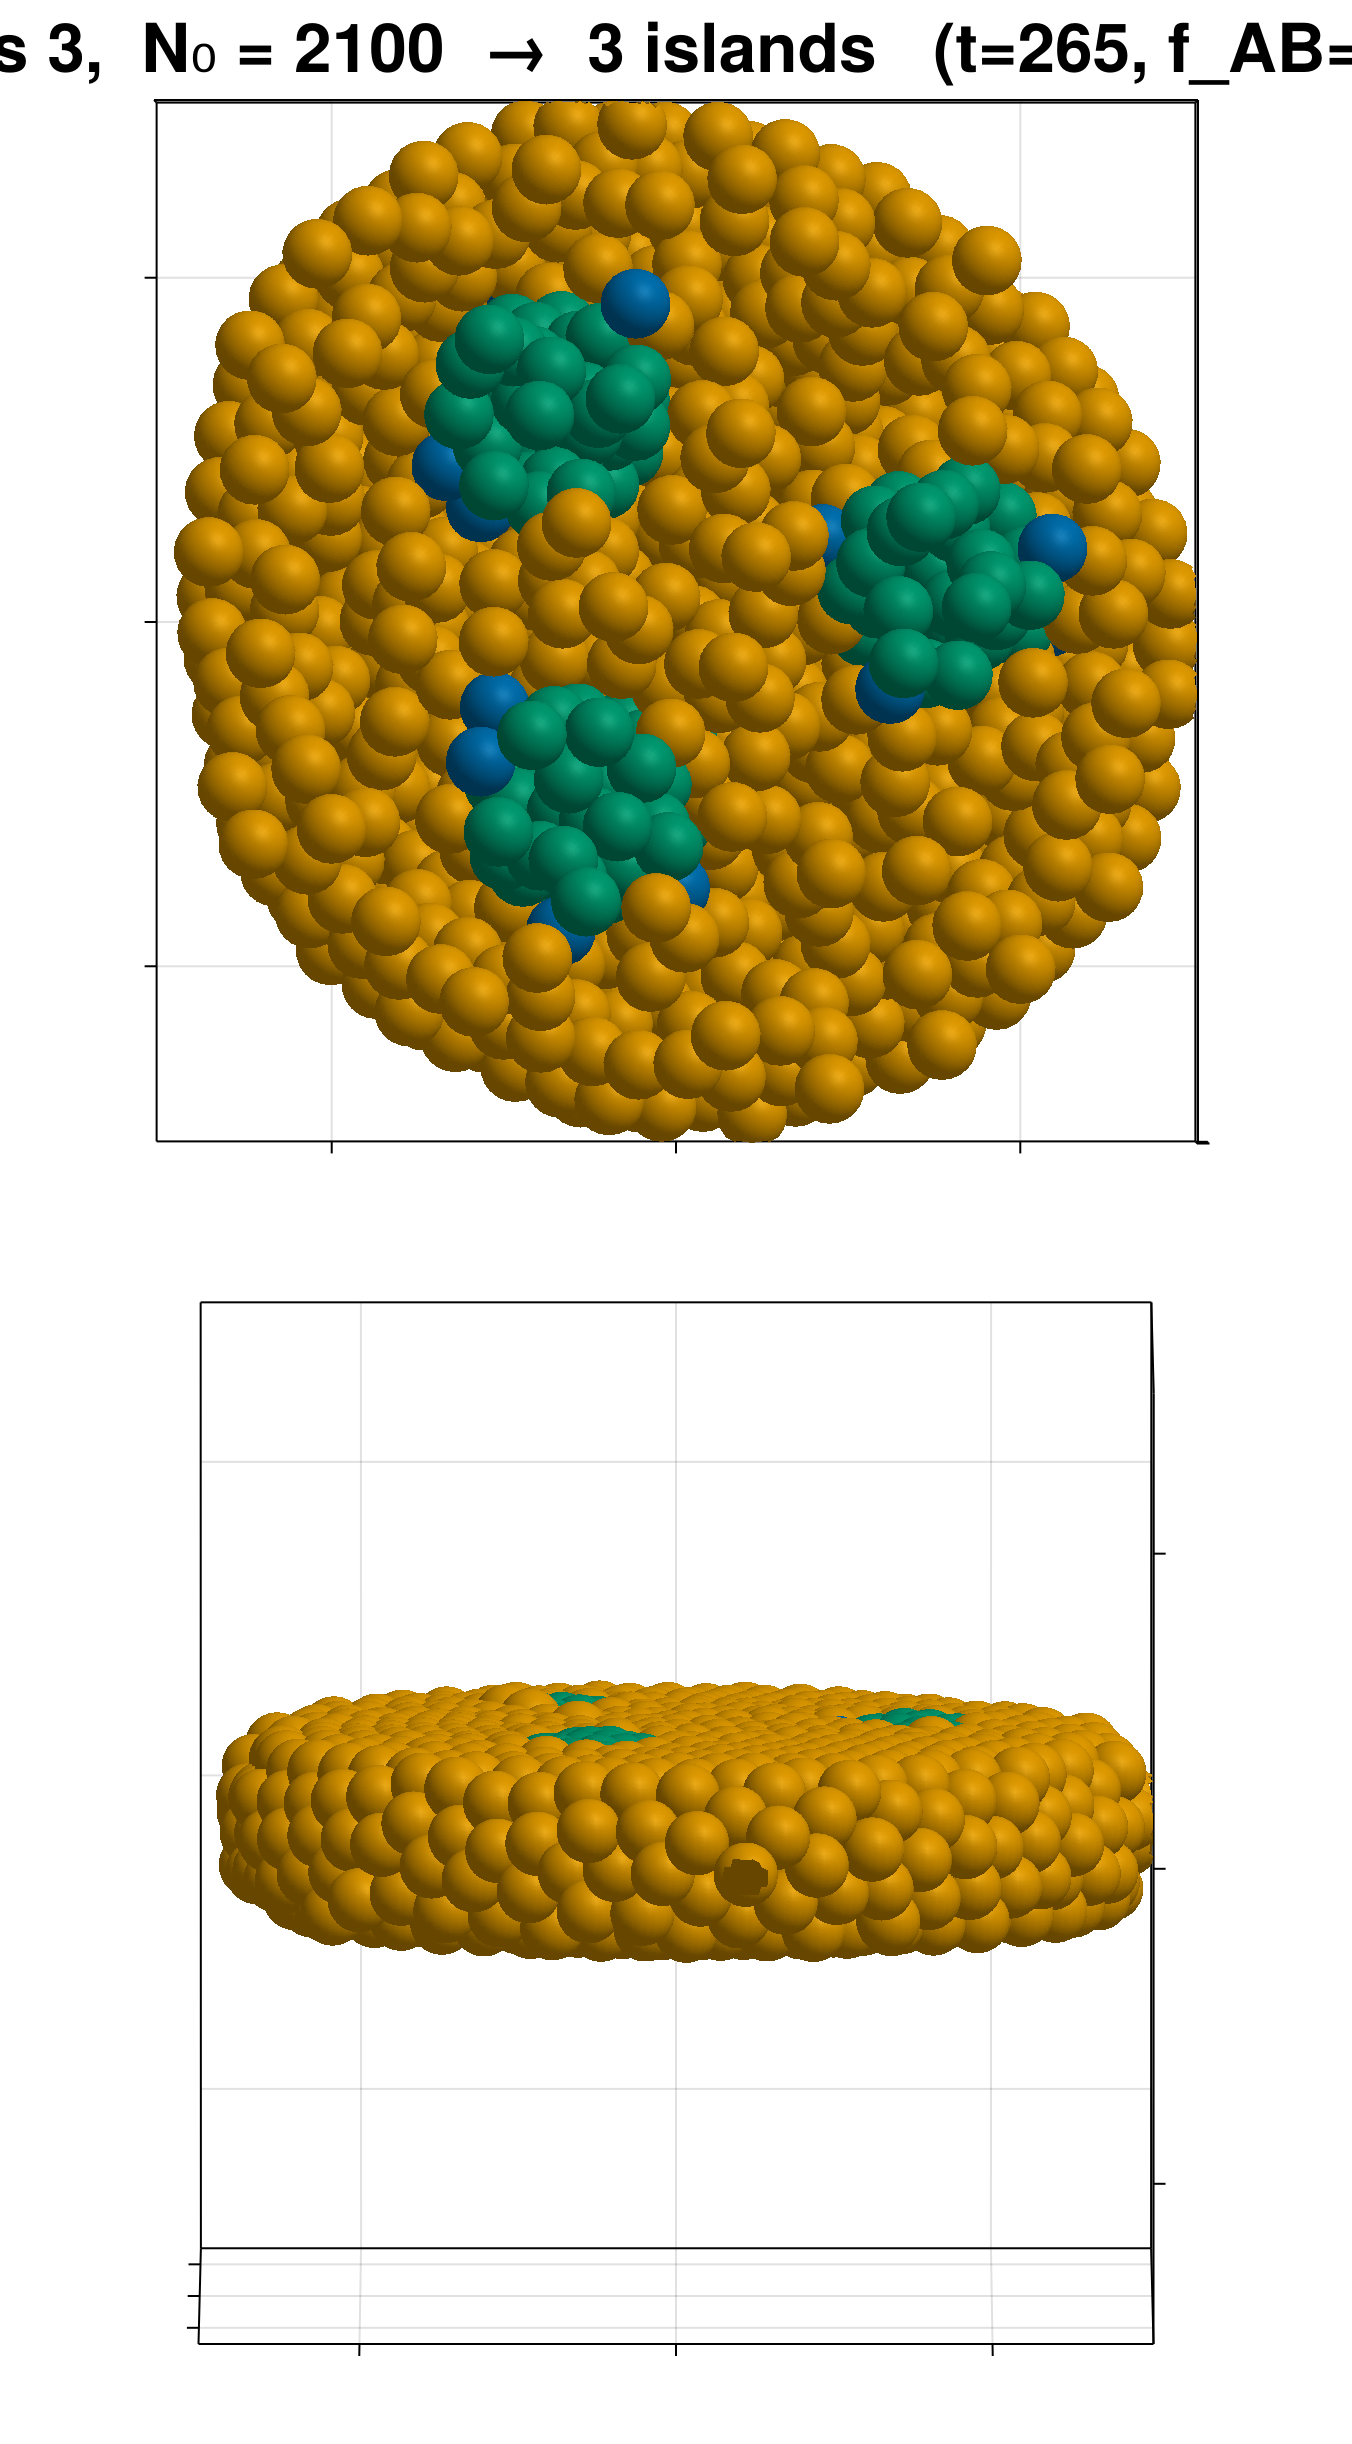
\includegraphics[width=0.2\linewidth]{figures/pattern_L3_islands_N2100.png}
    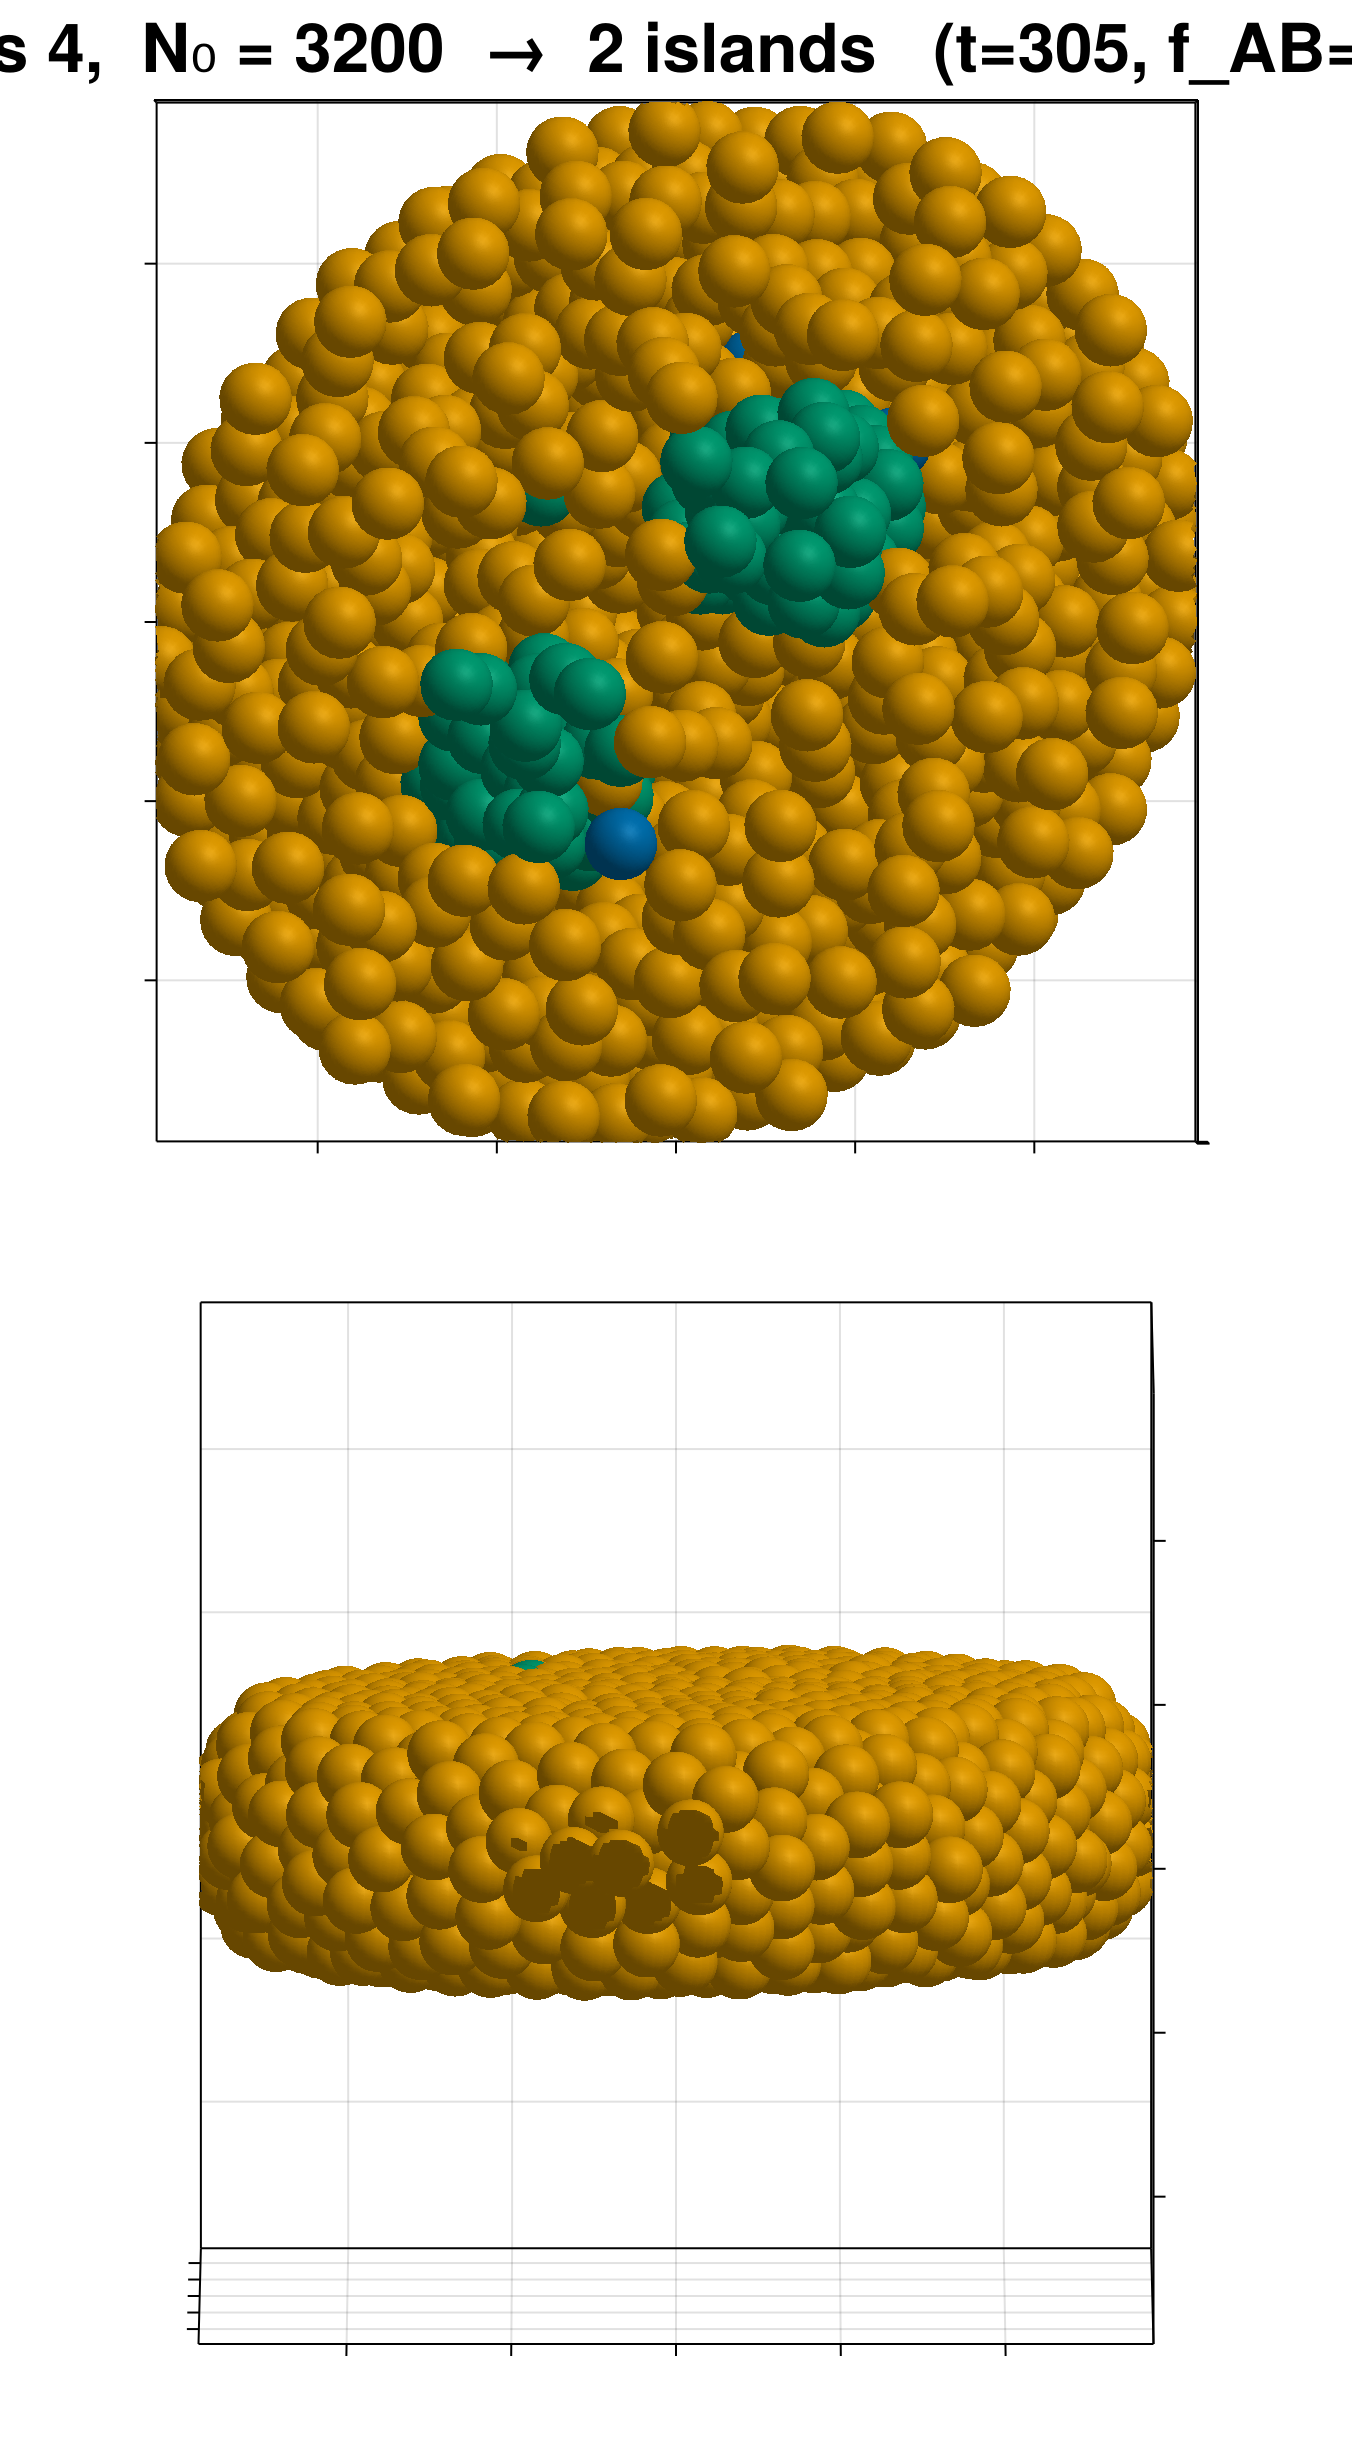
\includegraphics[width=0.2\linewidth]{figures/pattern_L4_islands_N3200.png}
    \caption{More concentred patterns for layers 1 to 4. Plot looks slightly uglier due to the engine used, and can be redone.}
    \label{final-patterns}
\end{figure}


\section{Adaptability and possible improvements}

I believe this should be adaptable to new rates of change $p,q$ relatively easily, since the algorithms for studying the correct functioning of the gastruloids (that is, polarisation, fusion, and patterning) are already established. Another possible change that we have discussed is considering local inhibition rates, which as far as I tested yield very similar results; at least we could try if it's preferred to have them that way.

The phase space plot could also be improved if you'd like to use it. I have two improvements in mind:
\begin{enumerate}
    \item Plot it in a more continuous fashion: instrad of considering layers 1,2,3,4,5, let it have values in between. I believe we could fit the transition curve and paint either side blue / green depending on the behaviour.
    \item Plot it in terms of the original radius on squeezing instead/apart from the initial N.
    \item Be clearer about the classification: "if we run 5 aggregates with the same parameters and get patterns 3 out of 5 times, do we classify it as patterns?".
\end{enumerate}



\newpage
\section{Parameters}

\begin{table}
{\small                                 % smaller font size for the table
\begin{xltabular}{\textwidth}{ 
    >{\centering\arraybackslash}p{0.12\textwidth}   % first column: 12% of text width
    X                                               % second column: take up the remaining space
    >{\centering\arraybackslash}p{0.15\textwidth}   % third column: 11% of text width
    >{\centering\arraybackslash}p{0.15\textwidth}   % fourth column: 11% of text width
}
\hline
\textbf{Symbol} & {\textbf{Description}} & \textbf{Value (code)} & \textbf{Value (exp)} \\      % header
\hline
    $\Delta t$ & Timestep & 0.02 & \\
    $ r$ & Radius & 1 & \\
     & Overlap factor & 0.3 & \\
    $\alpha$ & Cell-ECM/cell-cell friction parameter & 0.9 & \\
    $\tau_\text{div}^A$ & Average division time & 300 & \\
    $\tau_\text{div}^B$ & Average division time & 300 & \\
    $\tau_\text{div}^C$ & Average division time & 750 & \\
    $\sigma_\text{div}$ & Division time variability & 0.5 & \\
    $\lambda$ & Global friction coefficient & 1 & \\
    $\mu$ & Force range factor & $\begin{pmatrix}
        1.55 & 1.5 & 1.525 \\
        1.5  & 1.7 & 1.45 \\
        2.0  & 2.0 & 2.0
    \end{pmatrix}$ \vspace{0em} & \\
        & Neighbour range factor &  1 & \\
    $F_{rep}$ & Repulsion force & $\begin{pmatrix}
        3 & 3 & 3 \\
          & 3 & 3 \\
          &   & 5.1
    \end{pmatrix}$ \vspace{0em} & \\
    $F_{att}$ & Attraction force & $\begin{pmatrix}
        6 & 6 & 2.4 \\
          & 6 & 1.6 \\
          &   & 4.8
    \end{pmatrix}$ \vspace{0em} & \\
    $p$ & Fixed transition rate from $A$ to $B$ & 0.009333 & \\
    $q$ & Fixed transition rate from $B$ to $C$ & 0.004667 & \\
    $\lambda$ & Friction parameter & 1 & \\
    $K$ & Feedback parameter & 0.2 & \\
    $n_i$ & Number of neighbours &  & \\
    $n_i^X$ & Number of neighbours in state $X$ &  & \\
    $\phi_X$ & Proportion of cells in state $X$ &  & \\
    $T_0$ & Typical time scale & \SI{2}{\hour} & \\
    $R_0$ & Typical length scale & \SI{5}{\micro\meter} & \\
    $F_0$ & Typical force scale & \SI{20}{\pico\newton} & \\
\hline
\end{xltabular}
}
\label{parameters}
\caption{Base parameters used for the simulations.}
\end{table}

\end{document}